\documentclass[document.tex]{subfiles}
\begin{document}

\chapter{Background}
\section{Introduction}
\noindent Automatically solving Math Word Problem is a recently hot topic on understanding Natural Language. However, actual journey of solving was started from the 1960s. Algebraic problems of Natural Language was transformed into kernel sentences and handles to solve the problems in STUDENT\cite{4}. In CARPS\cite{5}, they use pattern matching based on expressions by the transformed kernel sentences. However, they were limited to rate based problems. In \cite{6}, they first introduced tree-based structure to represent the information in the problem. Recent automatically solving math word problems include number word problems\cite{7}, logic puzzle problems\cite{8}, geometry word problems\cite{9,10}, arithmetic word problems\cite{1}, \cite{11} and algebra word problems\cite{2,3}, \cite{12}.
\section{Parsing}
Parsing is the process of analyzing a string of symbols, either in natural language or in computer languages, conforming to the rules of a formal grammar. The term parsing comes from Latin pars (orationis), meaning part (of speech).

The term has slightly different meanings in different branches of linguistics and computer science. Traditional sentence parsing is often performed as a method of understanding the exact meaning of a sentence or word, sometimes with the aid of devices such as sentence diagrams. It usually emphasizes the importance of grammatical divisions such as subject and predicate.
Parsing are basically two types. One is \textbf{syntax analysis} and other is \textbf{semantic analysis}.

A \textbf{parser} is a software component that takes input data (frequently text) and builds a data structure – often some kind of parse tree, abstract syntax tree or other hierarchical structure – giving a structural representation of the input, checking for correct syntax in the process. The parsing may be preceded or followed by other steps, or these may be combined into a single step. The parser is often preceded by a separate lexical analyser, which creates tokens from the sequence of input characters; alternatively, these can be combined in scannerless parsing. Parsers may be programmed by hand or may be automatically or semi-automatically generated by a parser generator. Parsing is complementary to templating, which produces formatted output. These may be applied to different domains, but often appear together, such as the scanf/printf pair, or the input (front end parsing) and output (back end code generation) stages of a compiler. The overview of the parsing is shown in the figure below:
\begin{figure}[H]
	\begin{center}
		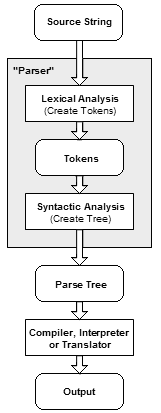
\includegraphics[height=13.0cm]{imgs/Parser.png}
	\end{center}
	\caption{Parsing Diagram}
	\label{fig:parsing}
\end{figure}
\section{Related to Semantic Parsing}
\noindent Semantic parsing is the process of mapping a natural-language sentence into a formal representation of its meaning. Semantics concerns its meaning: rules that go beyond mere
form (e.g., the number of arguments contained in a call to a
subroutine matches the number of formal parameters in the
subroutine definition – cannot be counted using Context Free Grammar, type
consistency):
\begin{itemize}
	\item Defines what the program means
	\item Detects if the program is correct
	\item Helps to translate it into another representation
\end{itemize}
In semantic parsing, there have been many works. Language grounding for interpretation of a sentence in world representation has related to many works \cite{13, 14, 15, 16, 17, 18, 19, 20, 21, 22, 23}. We discuss three pioneering work closely related to our work.
\section{Verb Categorization Technique}
\noindent In \cite{1}, they tried to solve addition and subtraction problems by verb categories to update a world representation derived from problem text. They ground the problem text to semantic entities and containers. Based on learned verb categories, their system works well for addition and subtraction.
They investigates the task of learning to
solve such problems by mapping the verbs in the
problem text into categories that describe their im-
pact on the world state. While the verbs category
is crucial, some elements of the
problem are irrelevant. For instance, the fact that
three kittens have spots is immaterial to the solution. 
%Overview of the process of verb categorization is shown below:
%\begin{figure}[H]
%	\begin{center}
%		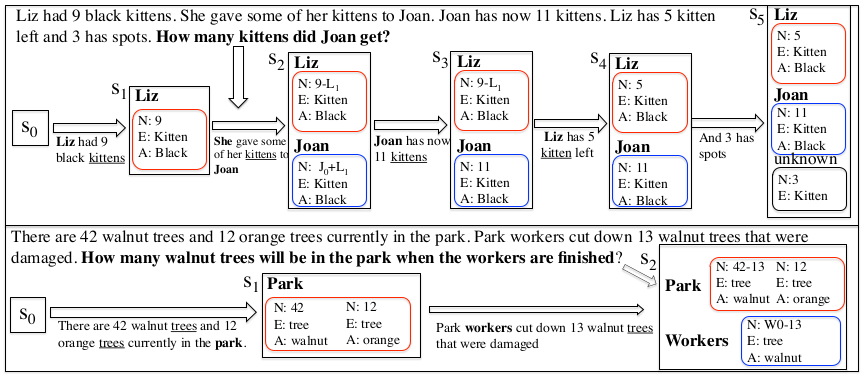
\includegraphics[height=10cm, width=16cm]{imgs/Verb.jpg}
%	\end{center}
%\end{figure}
\section{Template Matching Technique}
\noindent In \cite{2}, they introduce a general method for solving algebra problems. This work can align a word problem to a system of equations with one or two unknowns. They learn a mapping from word problems to equation templates using global and local features from the problem text. However, the
large space of equation templates makes it challenging for this model to learn to find the best equation
directly, as a sufficiently similar template may not
have been observed during training.
\section{Hybrid of Verb Categorization and Template Matching Technique}
\noindent In ALGES\cite{3}, they tried to solve the problem of solving multiple sentenced algebraic word problems by generating and ranking the equation trees. They use a richer semantic representation of the problem text and a bottom-up approach to learning the relations between spans of texts and arithmetic operators. Then score the equations using a global form of the problem to produce the final result. ALGES combined the previous methods to use in broader scope like, Addition, Subtraction, Multiplication and Division for solving single variable problems.

ALGES learns to map spans of text to arithmetic operators, to combine them given the global context of the problem, and to
choose the “best” tree corresponding to the problem.
The training set for ALGES consists of unannotated
algebraic word problems and their solution. Solving the equation represented by such a tree is trivial.
ALGES is able to solve word problems with single-variable equations.
In contrast to \cite{1} ALGES covers $ +, -, *, $ and $/$. The work of \cite{2} has broader scope but we show that it relies heav-
ily on overlap between training and test data.
\section{Conclusion}
\noindent Our work is related to ALGES, where we converted the percent related number to a fraction and force the problem text to covert it like the problem for ALGES. That is related to using ILP to enforce global constraints in NLP applications\cite{24}. Like previous\cite{25, 26, 27, 28}, ALGES used ILP to form candidate equations which are then used to generate training data for classification. ALGES attempts to parser re-rank the equations\cite{29, 30}.

%\begin{figure}[H]
%        \centering
%        
\includegraphics[width=3in]{imgs/camera.jpg}
%        \caption[A Camera]
%        {A Camera}
%\end{figure}
%
%\noindent Lorem ipsum dolor sit amet, consectetur adipiscing elit, sed do eiusmod tempor incididunt ut labore et dolore magna aliqua. Ut enim ad minim veniam, quis nostrud exercitation ullamco laboris nisi ut aliquip ex ea commodo consequat. Duis aute irure dolor in reprehenderit in voluptate velit esse cillum dolore eu fugiat nulla pariatur. Excepteur sint occaecat cupidatat non proident, sunt in culpa qui officia deserunt mollit anim id est laborum.
%
%\begin{figure}[H]
%        \centering
%        \begin{subfigure}[b]{0.4\textwidth}
%                
\includegraphics[width=\textwidth]{imgs/typewriter.jpg}
%                \caption{A Typewriter}
%                \label{fig:typewriter}
%        \end{subfigure}
%        \begin{subfigure}[b]{0.4\textwidth}
%                
\includegraphics[width=\textwidth]{imgs/macbookpro.jpg}
%                \caption{A Macbookpro}
%                \label{fig:macbookpro}
%        \end{subfigure}
%        \caption{Typewriter and Macbookpro}\label{fig:typewriter_macbookpro}
%\end{figure}

\end{document}
